\chapter{Background and Motivation}
\label{chap:background}

\emph{insert description of what background contains}

\section{RUM}
insert info about RUM here. 

\section{R-trees}
R-trees was first presented in 1984 by Antonin Guttman\cite{r-tree} and was created to better handle indexing and retrieval of multi-dimensional data by their spatial locations. Previous solutions such as B+-trees are not equipped to handle data with multiple dimensions as they only support one-dimensional index structures \cite{ComparisonOfAdvancedTree}. R-trees are structured as a hierarchy with a root node which points to lower nodes until you reach the leaf nodes which contain pointers to where the objects are stored. To be able to store multi-dimensional data objects R-trees use n-dimensional rectangles to index objects according to a certain space. These rectangles are known as \emph{Minimum Bounding Rectangles} (MBRs) and each root or intermediate node points to the MBRs that is contained within the MBR stored in the intermediate node. In the general R-tree, each intermediate node will contain distinct MBRs, even if they are present in several. Each non-leaf node is represented in the tree by (\emph{MBR},  \emph{p}) where \emph{MBR} is the minimum bounding rectangle which spatially contains all MBRs in the child node, and \emph{p} is a pointer to a child node. The leaf-nodes is represented by (\emph{MBR}, \emph{o}) where \emph{MBR} is the minimum bounding rectangle which spatially contains the object, and \emph{o} is the object identifier. The height of the R-tree is at most \(log_mN-1\), when containing N index records. \emph{M} is the maximum number of entries that will fit in one node, and \emph{m} is the minimum number of entries in a node given by \(m <= M/2\). An example of an R-Tree structure can be seen in Figure \ref{fig:RTree} and Figure \ref{fig:RtreeSpace}.



\begin{figure}[ht]
    \centering
    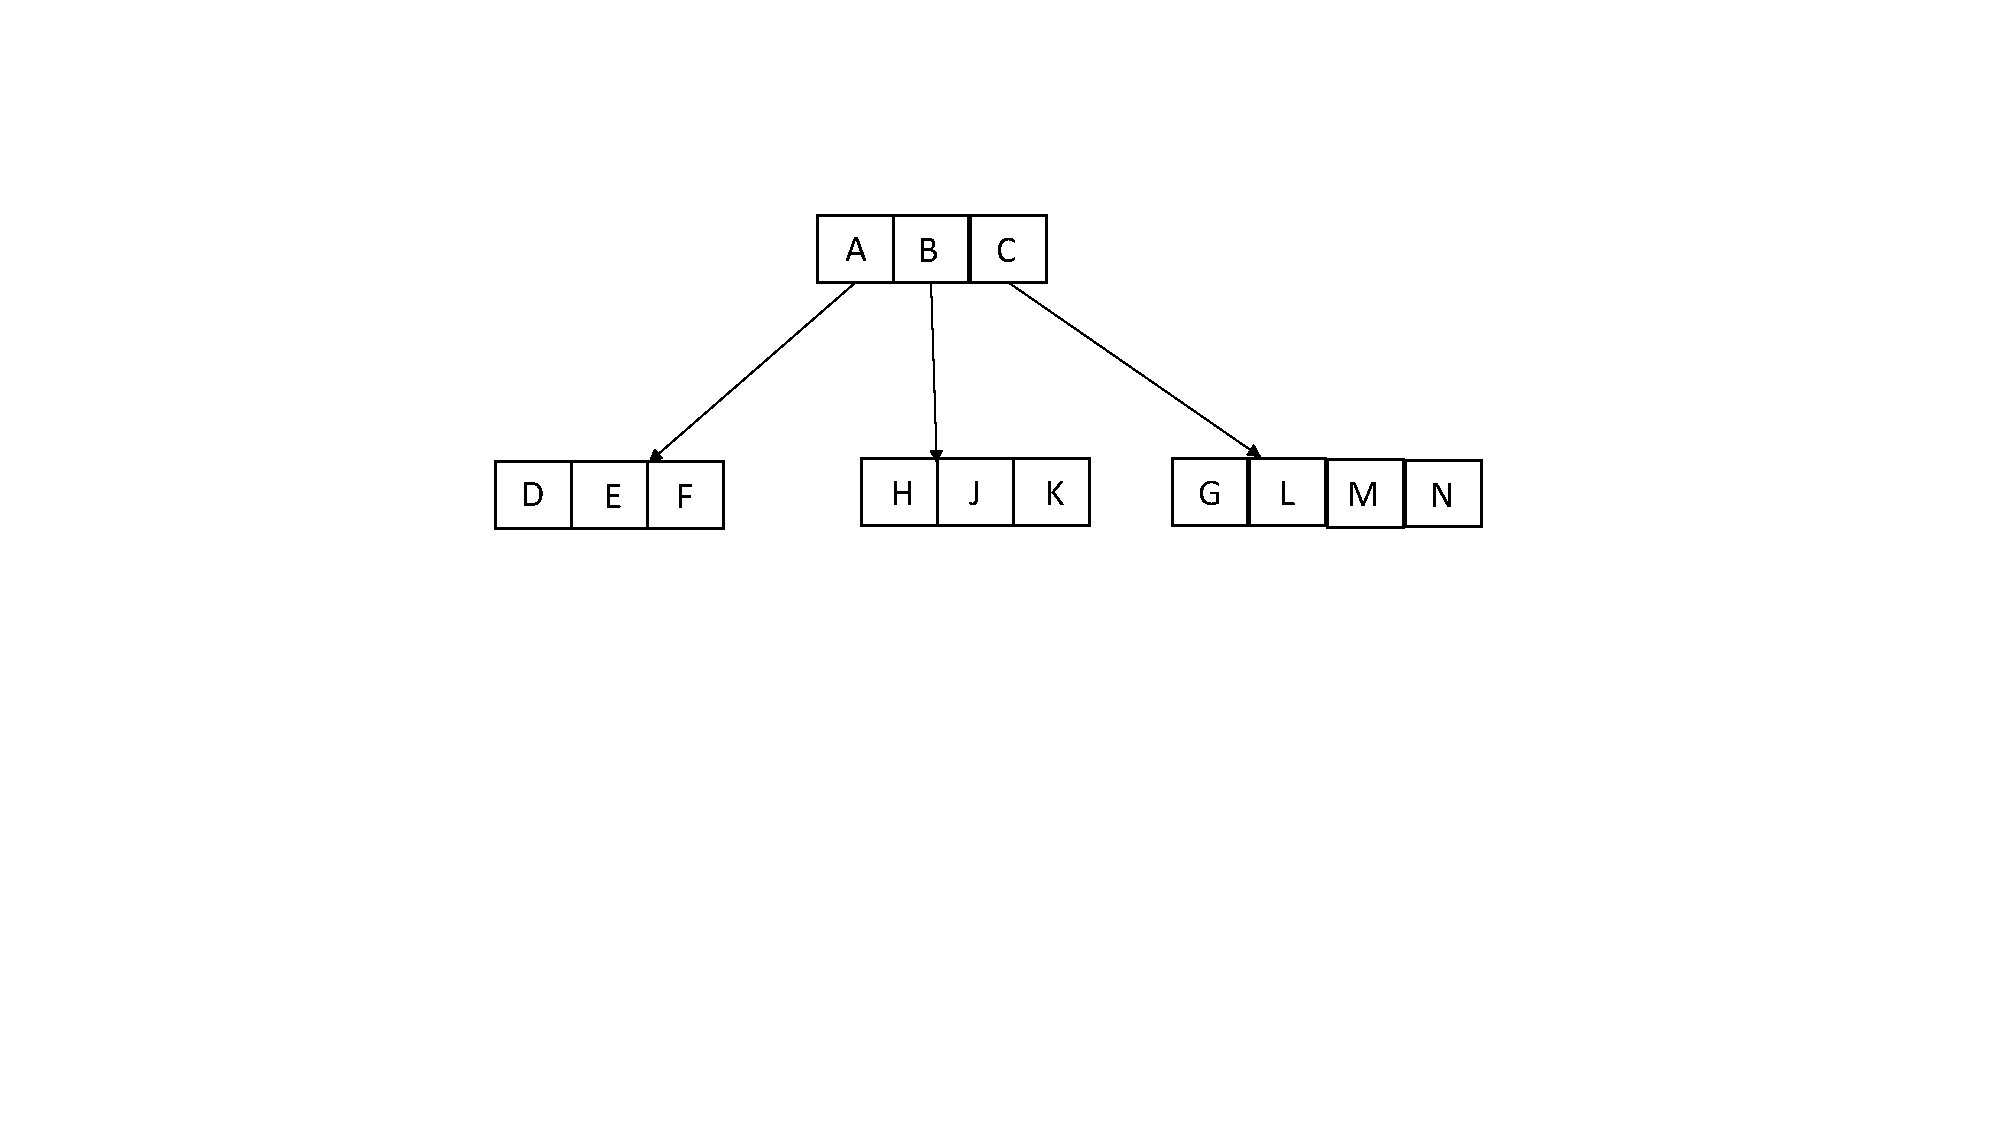
\includegraphics[scale=0.4]{figures/RTree.pdf}
    \caption{R-Tree index structure}
    \label{fig:RTree}
\end{figure}

\begin{figure}[ht]
    \centering
    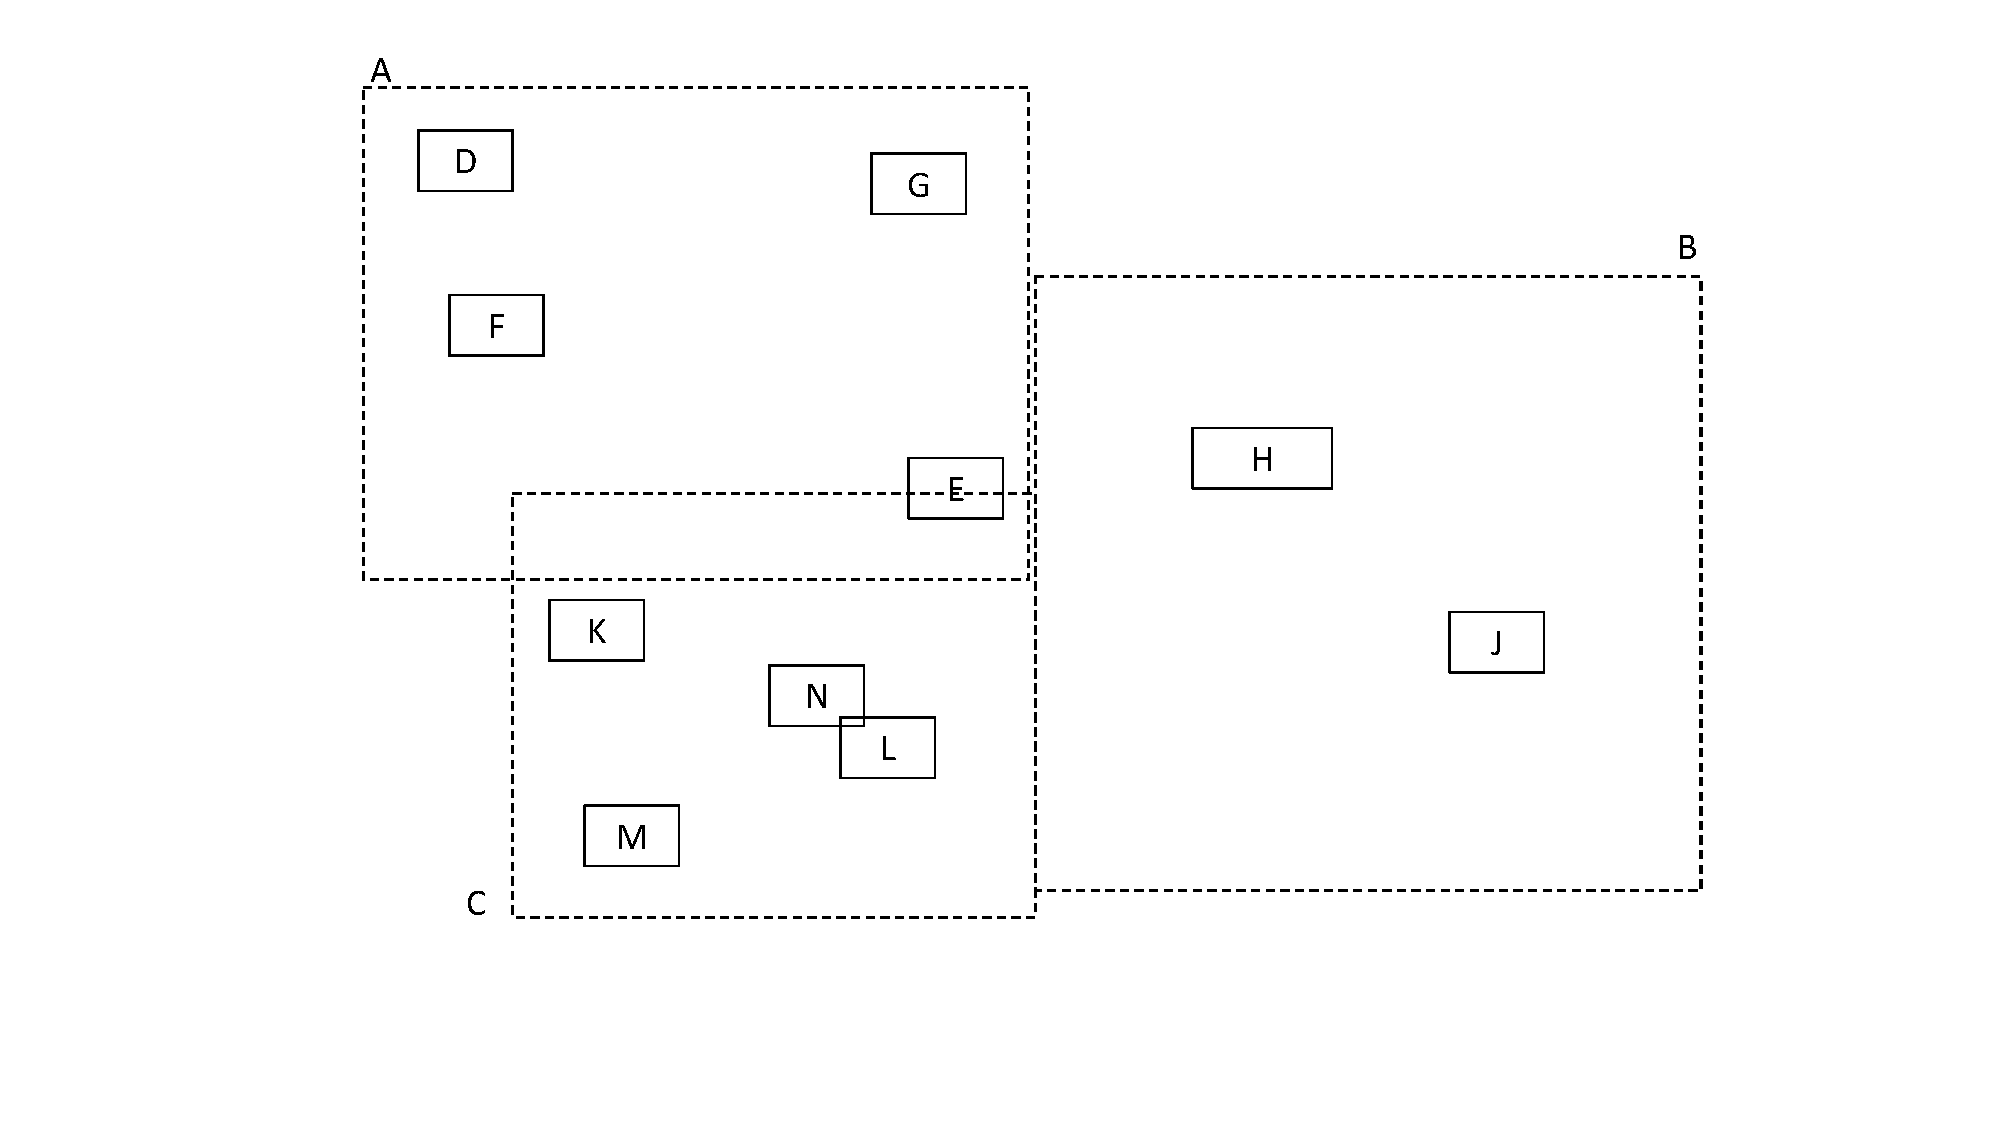
\includegraphics[scale=0.3]{figures/r-tree_space.pdf}
    \caption{R-Tree space structure}
    \label{fig:RtreeSpace}
\end{figure}

\subsection{Searching}
Search in R-trees are done in a similar way as with B-trees. The search is done by creating a search rectangle \emph{SR}, and checking all entries in the root node that contains MBRs that overlap with SR. A further search is done by traversing the subtree of the matching entries until all leaf node MBRs that overlap with SR are found. In worst-case scenarios this will lead to the whole tree being searched before finding a match. 

\subsection{Insertion}
Insertions in R-trees are done by inserting the new entry in a leaf node. This is done by searching the tree from the root node and finding the subtrees that overlap with the insertion entry. When the suitable node is found in at the leaf level, the entry is placed if there is enough space in the node. If the node is full, which would lead to overflow, the node is split and the tree is adjusted upwards to suit the new index structure. The leaf node which has the least need for enlargement to fit the new entry is chosen.

\subsection{Deletion}
Deletion is done by first finding the leaf node that contains the entry that is to be deleted. This is done by checking which parts of the tree overlaps with the entry, and when the correct leaf node is found, the entry is removed. After the removal, the remaining leaf node is checked to see if it has too few entries and will need to be readjusted. If this is the case, the tree will be restructured so that each leaf node meets the requirement of having a minimum of \emph{m} entries. 

\subsection{Splitting}
Splitting is a crucial part of the R-tree as it is used when inserting entries into full nodes and different methods can have a big impact on the search time. An important part of splitting is making as small rectangles as possible for the two new MBRs created by the split. This is to avoid searching the MBRs without results, which could be the case if the rectangles contain a lot of "empty" space which in turn could overlap with the search rectangle. The splitting methods \emph{Exhaustive Split}, \emph{Quadratic Split} and \emph{Linear Split} are presented by Guttman \cite{r-tree}. In his paper he finds that the linear split method is as good as the more expensive methods without affecting the search performance to an important extent. The quadratic split method is however said to have better overall performance as stated by Beckmann, Kriegel, Schneider and Seeger\cite{R*-tree}.

\subsubsection{Exhaustive Split}
This method executes all possible splits and then chooses the split with the MBRs that cover the underlying rectangles with the least redundant space and smallest overlap. The exhaustive split is the optimal solution, however it is computationally heavy to perform and the number of possible splits is potentially very large.

\subsubsection{Quadratic Split}
The quadratic split is executed by finding the two entries that will create a new rectangle wich fills the most space. These two entries are then put in two separate MBRs, before each remaining entry from the original node is put in one of the new MBRs by finding which will enlarge it least. If one of the MBRs will contain less than \emph{m} entries if not all remaining entries are assigned to it, then the remaining points are assigned to that MBR. The cost of this method is quadratic in M, as each entry will have to be computed with each other entry when finding the largest space to do the first split. 

\subsubsection{Linear Split}
The linear split is executed similarly as the quadratic split. However, instead of finding the space between each entry, it only finds the distance between the most extreme rectangles. Extreme rectangles are the ones that are the farthest on each side for the x-axis. This distance is normalized by taking the width, which is the length between the outer sides of the extreme rectangles. In the end, the pair with the highest value is chosen and put into two new MBRs. The remaining entries are put in the new MBR that require the least enlargement. The cost of this method is linear in M. 

\subsection{R+-tree}
The R+-tree is a variant of the general R-tree and was introduced in 1987 by Sellis, Roussopoulos and Faloutsos \cite{R+Tree}. It was developed to avoid overlapping MBRs in intermediate nodes. In the general R-tree each intermediate node contains MBRs which completely covers the MBRs in the child nodes. This can lead to all nodes having to be searched for a specific data object, which is not optimal. To reduce the number of intermediate nodes to be searched, the R+-tree splits the MBRs in intermediate nodes which point to leaf nodes. This is done so these MBRs do not overlap, and instead the MBRs at leaf level can be stored in multiple nodes. An important thing to note however is that the improved search performance of R+-trees has a negative effect on the space utilisation. This is however minimal if search performance is an important factor in the use of the R-tree index. 

\subsection{R*-tree}
The R*-tree is an extension of the general R-tree which is attractive as it supports both point and spatial data without increasing the implementation cost too much. This structure was presented in 1990 by Beckmann, Kriegel, Schneider and Seeger\cite{R*-tree}. In this paper they discuss the different parts that are essential for retrieval performance.\newline

\textbf{The area covered by intermediate MBRs should be minimised}\newline
The "empty" space covered by bounding rectangles should be minimized to avoid additional access paths when conducting a search. \newline

\textbf{The overlap between intermediate MBRs should be minimised}\newline
When minimizing the overlap, the possible access paths during a search is also minimized. \newline

\textbf{The margin of intermediate MBRs should be minimised}\newline
The margin of a bounding rectangle is the sum of the rectangle sides length. Minimization of the margin will lead to more quadratic shaped rectangles, which in turn are easier to place in space without causing overlap. This will again make it easier for the parent MBRs to reduce their size. \newline

\textbf{Storage utilisation should be optimised}\newline
With higher storage utilisation, the height of the tree will be reduced which will lead to lower query costs. \newline


An important thing to note is that it is difficult to achieve both high storage utilisation when also minimising the area covered by each MBR and their overlap. This is because the shape of the rectangles and the number of entries in each node needs to be more relaxed. Reducing the margin will however most likely lead to better storage utilisation. \newline

In order to improve the retrieval performance, the R*-tree focuses on the insertion of new rectangles. When choosing the subtree for insertion, the structure focuses on finding the path wich leads to the least need for \emph{overlap} enlargement to include the new entry. This is in contrast to the general R-tree where it decides based on the least need for area enlargement in total. If a leaf node is full the algorithm uses reinsertion if it is the first overflow at that particular level in the tree. Reinsertion is coslty, but gives better query performance than node splitting. If a reinsertion has already been used on a level, a splitting method is applied. The splitting method consists of deciding a split axis among all dimensions and choosing the division of entries that lead to the least overlap between the resulting MBRs.

\subsection{Dynamic Hilbert R-trees}
Hilbert-curve is a space filling curve, shown to achieve the best clustering when compared to Z-order and Gray-code curve \cite{HilbertRTree}. The Hilbert R-tree is constructed to behave like a R-tree on search, and a B*-tree during splitting on insertion. This is done by using a method called \emph{2D-c}, which sorts the data rectangles based on the 2d-hilbert value of their centers. Leaf nodes contains the same as with a regular R-tree (MBR, o), while non-leaf nodes contain addiotional information about the \emph{Larges Hilbert Value} (LHV) as (MBR, p, LHV). LHV is the largest hilbert value found in the MBRs enclosed by the non-leaf node's MBR. With insertion, the Dynamic Hilbert R-tree uses a method like is done in B*-trees. In regular B-trees splitting a node is done when it overflows, and two nodes is created from the overflowed node. In B*-trees the splitting is delayed by trying to send entries to sibling nodes when the original node is overflowed. The number of siblings can be chosen as \emph{s}, and when all sibling nodes are full, the split will be conducted by creating \emph{s+1} nodes to handle the overflow entry. The best tradeoff for choosing siblings is shown to be 3-to-4 splitting, which entails having three siblings. This gives the best insertion speed, which decrease with the increase of siblings, while maintaining a good performance, which increase with the number of siblings. 

In the original presentation of the Dynamic Hilbert R-tree it is shown that it outperforms R*-trees on response time by up 28\%\cite{HilbertRTree}. It has however later been discovered that the Dynamic Hilbert R-tree is vulnerable to large objects performance-wise. In addition the proximity is not kept to a satisfying degree by the Hilbert curve as the space dimensionality increaes, which leads to MBRs overlapping more in internal tree nodes\cite{RTreesTheoryApplications}.


\section{The Log-Structured Merge-Tree}
The \emph{Log-Structured Merge-tree} was introduced in 1996 by O'Neil, Cheng, Gawlick and O'Neil\cite{LSMTree}. It is a write-optimized storage structure created to handle big amounts of insertions, while still being able to search for entries by index. The structure of LSM-trees consists of multiple levels. The top level is in memory, known as $C_0$ where entries are stored in a tree by index. The lower levels $C_1, C_2 ... C_n$ are stored on disk and store its entries in a B-tree like index structure. Instead of inserting one entry at a time, the LSM-tree loads entries to disk in batches by using a method called \emph{rolling merge}. The in-memory component $C_0$ is smaller than the lower components, while the lever components grow in size the further down they are in the chain. When $C_0$ reaches a treshold close to its maximum size, entries are sent to merge with $C_1$ while a batch of entries from $C_1$ are put in a buffer. The block containing the old entries from $C_1$ before merge is called the \emph{emptying} block, while the new leaf nodes merged from $C_0$ is called the \emph{filling} block. The filling block is stored on a new disk page to keep the old entries in case recovery is needed. This means that write operations are done in-place in $C_0$, while they are done out-of-place in the lower components. The structure of LSM-trees with two levels can be seen in figure \ref{figure}, while the rolling merge process can be seen in figure \ref{fig:LSMMerge}. 

\begin{figure}[ht]
    \centering
    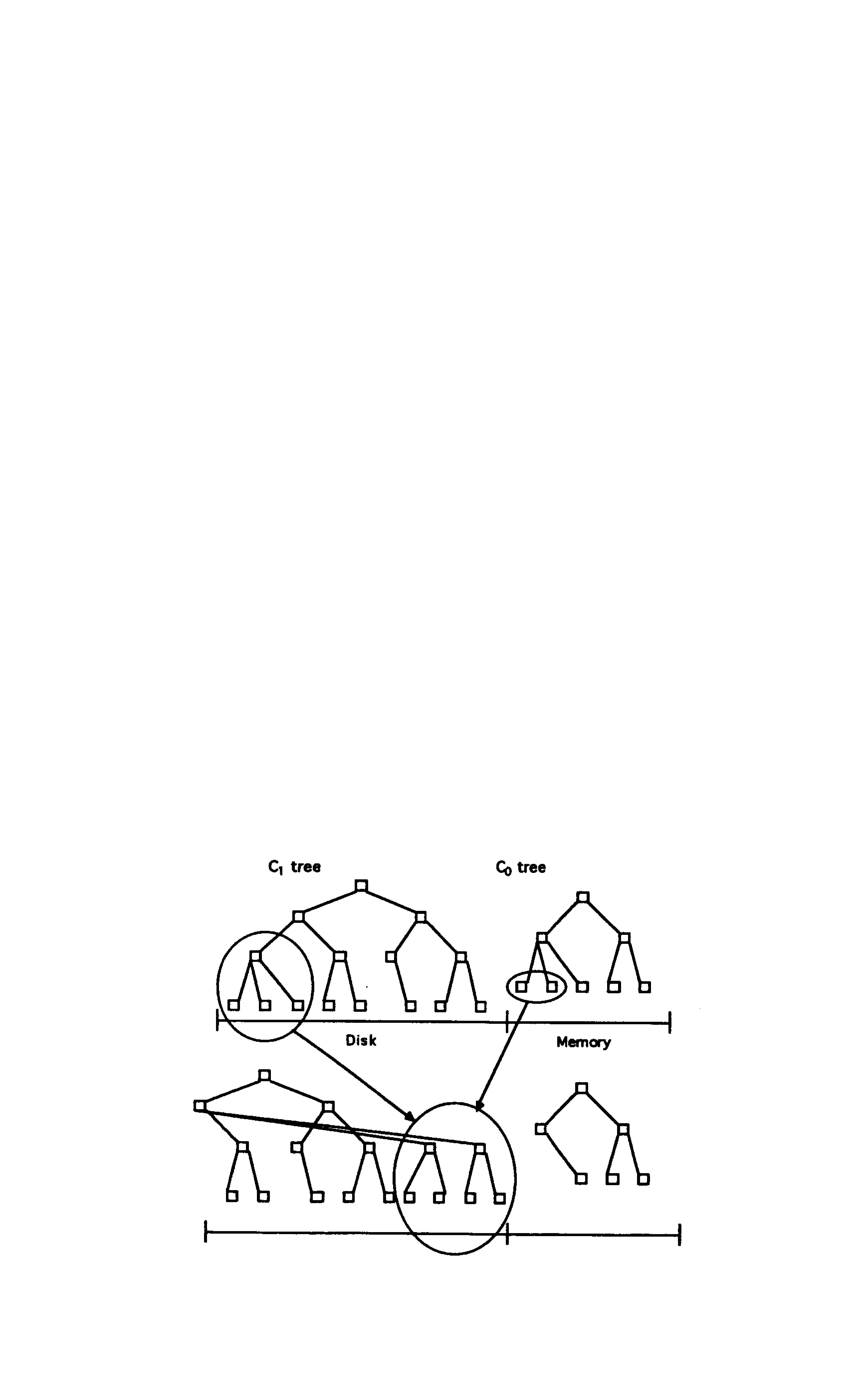
\includegraphics[scale=0.7]{figures/merge_LSM.pdf}
    \caption{Rolling merge\cite{LSMTree}}
    \label{fig:LSMMerge}
\end{figure}

Delete operations in the Log-Structured Merge-tree is processed by first searching for the entry in $C_0$. If it is found it is removed, if it is not present a \emph{delete node entry} is created and placed by index and noting an entry row to delete. This block is then sent through the levels by following the rolling merge method as is done with insertions. Updates are handled by first deleting an entry and then inserting a new one.
\newline

An important part of optimising the LSM-tree is to find the most suitable sizes for the different components. The size of the in-memory component $C_1$ can be costly if it is too big, but must be big enough to decrease the amount of I/O operations needed to move entries to disk. The ratio between the sizes of $C_0$ and $C_1$ is given by $1/M$, where \emph{M} is the average number of entries merged during the rolling merge process between the two. The LSM-tree is originally designed with magnetic hard drives in mind, using sequential writes to optimize the use of the disk arm. This is however also a good solution for solid state drives (SDDs), as there is not a big gap performance-wise between sequential and random writes. In addition, the use of out-of-place updates is well suited as SSDs are prone to wear-down\cite{LSMSDD}.

\subsection{Today's LSM-trees}
The structure of LSM-trees have evolved over time, and is now widely used by different NoSQL systems such as Cassandra\cite{Cassandra} and Bigtable\cite{Bigtable}. The basic structure of the LSM-tree used today is similar to the one described in 1996 \cite{LSMTree}, but instead of merging higher levels into components in the lower levels, components are merged together into a new one instead\cite{LSMSurvey}. In addition to B+-trees, \emph{Sorted-String Tables} (SSTables) are often used as index structures. SSTables is made up of a list containing data blocks storing key-value pairs ordered by key, and an index block storing the key range for that list. 

\subsubsection{Merging policies}

The increase in number of components causes lower query performance, which is adressed by using merging methods to reduce them. \emph{Leveling} and \emph{Tiering} are two merge policies used in practice. Each policy organise disk componts into logical levels or tiers which are sized after a ratio \emph{T}. In the leveling merge policy, there is only one component per level and each component is \emph{T} times larges than the level above it. Entries from the upper level will therefore be merged multiple times with its sub-level, until the sub-level is full and then merged further down. The tiering merge policy has \emph{T} components per level. When a level is full, all of its components are merged together into a new component at the level below. The tiering merge policy is optimised for a high write-load, while the leveling merge policy is better performance-wise for query performance as the number of components to search is more reduced\cite{LSMSurvey}. 

\subsubsection{Challenges}
\textbf{her må du undersøke hva du må linke til. De forskjellige metodene for å forbedre ting er nevnt i artikkelen LSMSurvey. Spør SE hvordan dette burde løses.}

With today's LSM-trees there are still areas that can be improved. \newline

\emph{Write amplification} is an issue as data has to be written multiple times when sending it through levels for merging. This can in the long run lead to wear-down of disk pages in SSDs. This is however improved with the use of the tiering merge policy as it has better write performance. There also exists methods trying to improve this such as merge skipping, which skips levels when merging data down through the levels, hash-partitioning to distribute the data evenly and exploiting data skew by keeping track of hot and cold entries and only sending cold entries to disk. Keeping the hot entries in memory saves write operations as they can be written over directly. \newline

\emph{Merge operations} are an important part of LSM-trees, and can lead to buffer cache misses and write stalls when large merge operations are processed. Examples of improving the merge performance can be to check if a page from an SSTable overlaps with any of the pages in the SSTable it is to be merged with. If not, the resulting SSTable can contain pointers instead of having to read and write the pages during merge. Another method is to use pipelining during the merging process, as it is CPU-based. By doing this, the CPU is utilised in a more effective manner. To avoid buffer cache misses external servers can be used for large merge operations or the old SSTable (before merge) can be stored in a buffer in the underlying level. This is however mainly effective on skewed workloads as storing cold pages additionally is not optimal. To minimize write stalls the write-throughput can be limited by only allowing a merge operation in a level to continue if the previous merge operation in that level has finished. \newline

\emph{Hardware} has evolved since LSM-trees was first introduced. As LSM-trees was designed based on magnetic hard drives it is important to find ways to find better ways to utilize the new storage devices and their benefits. \newline

\emph{Special workloads} also have an effect on the structure of LSM-trees. The distribution can for example be a factor that should be taken into account when deciding the implementation. \newline

\emph{Auto-tuning} is mostly ways of optimising the LSM-tree for the intended use. As explained in the RUM conjecture\cite{insert RUM}, access methods cannot be read- write and space-optimal at the same time. The different ways of tuning the LSM-tree can therefore be a great way to adapt to different workloads and in which ways they are handled. A challenge with auto-tuning is that there are many different aspects to tune, such as choosing the correct merge policy and finding the correct size ratio between components.
